\chapter{}\label{ch:auf5}
Das Ziel der Aufgabe ist es, die Drehzahl- Drehmomentkennlinie für den BLDC für die Ankerspannungen 
\begin{center}
	$ U_{AP} = 10V $\hspace{1cm}$ U_{AP} = 15V $\hspace{1cm}$ U_{AP} = 20V $\\
\end{center}
zu messen. Die Belastung des Motors erfolgt durch Einstellung eines geeigneten Laststroms $ I_{AL} $ in der Bedienoberfläche am Labor- PC.

\section{}\label{sec:5a}
Es sollen jeweils die Messungen der Drehzahlen für die Drehmomente $ M_{L} = M_{Mi} $
\begin{center}
	$ M_{L} = 0 Nm $ \hspace{0.7cm} $ M_{L} = 0,05 Nm $ \hspace{0.7cm}	$ M_{L} = 0,1 Nm $ \hspace{0.7cm}	$ M_{L} = 0,15 Nm $ \hspace{0.7cm}	$ M_{L} = 0,2 Nm $
\end{center}	
durchgeführt werden. Anschließend sind diese grafisch darzustellen. Die Drehmomente sind über den Laststrom $ I_{AL} $ einzustellen, dafür wird Formel \ref{eq:1b:ML} nach $ I_{A} $ umgestellt:
\begin{equation}
	I_{A}(M_{L}) = \frac{M_{L}}{C_{M}\Psi_{PML}} = \frac{M_{L}}{\frac{C_{E}}{2\pi}\Psi_{PML}}
	\label{eq:5a:IA}
\end{equation}
Die hierdurch ausgerechneten Werte sind in Tabelle \ref{tab:5a:Drehzahlen} zu sehen. Anschließend wird der Prüfstand auf die entsprechenden Umgebungsparameter eingestellt und die resultierenden Drehzahlen protokolliert.
\begin{table}[h]
	\centering
	\begin{tabular}{p{2cm} | p{2cm} | p{2cm} p{2cm} p{2cm} | p{2cm} }
		&&&&&\\[-1em]
		$ M_{L} $ & $ I_{A}(M_{L}) $ & $ U_{AP} = 20V $ & $U_{AP} =  15V $ & $U_{AP} =  10V $ & $ R_{L} = 1\Omega $ \\
		\hline &&&&&\\[-1em]
		$ 0Nm $ & $ 0A $ & 3030 & 2270 & 1550 & 0 \\
		$ 0.05Nm $ & $ 0,79A $ & 2727 & 2025 & 1295 & 164 \\
		$ 0.1Nm $ & $ 1,57A $ & 2486 & 1806 & 1100 & 330 \\
		$ 0.15Nm $ & $ 2,36A $ & 2174 & 1530 & 855 & 495 \\
		$ 0.2Nm $ & $ 3,14A $ & 1906 & 1281 &   & 660
	\end{tabular}
	\caption{Drehzahl in Abhängigkeit des Lastmoments $ M_{L} $ und Ankerspannung $ U_{AP} $} in $ min^{-1} $
	\label{tab:5a:Drehzahlen}
\end{table}

\section{}\label{sec:5b}
Es ist die entsprechende Kennlinie in das gemessene Drehzahl-Drehmomentkennlinienfeld für $ R_{L} = 1\Omega $ einzutragen. Dazu werden die oben genannten Lastmomente in die Formel \ref{eq:1c:NP} eingesetzt.
\begin{figure}[h]
	\centering
	% This file was created by matlab2tikz.
%
%The latest updates can be retrieved from
%  http://www.mathworks.com/matlabcentral/fileexchange/22022-matlab2tikz-matlab2tikz
%where you can also make suggestions and rate matlab2tikz.
%
\definecolor{mycolor1}{rgb}{0.00000,0.44700,0.74100}%
\definecolor{mycolor2}{rgb}{0.85000,0.32500,0.09800}%
\definecolor{mycolor3}{rgb}{0.92900,0.69400,0.12500}%
\definecolor{mycolor4}{rgb}{0.49400,0.18400,0.55600}%
%
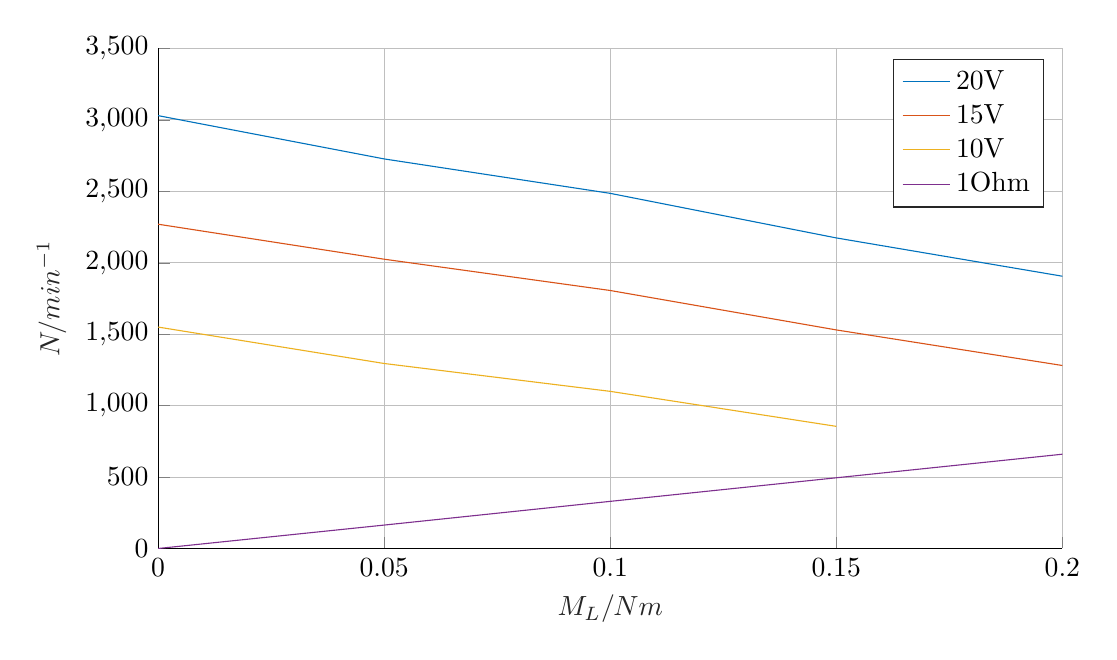
\begin{tikzpicture}

\begin{axis}[%
width=4.521in,
height=2.5in,
at={(0.758in,0.481in)},
scale only axis,
xmin=0,
xmax=0.2,
xtick={   0, 0.05,  0.1, 0.15,  0.2},
xticklabels={{0}, {0.05}, {0.1}, {0.15}, {0.2} },
xlabel style={font=\color{white!15!black}},
xlabel={$ M_{L}/Nm $},
ymin=0,
ymax=3500,
ylabel style={font=\color{white!15!black}},
ylabel={$ N/min^{-1} $},
axis background/.style={fill=white},
axis x line*=bottom,
axis y line*=left,
xmajorgrids,
ymajorgrids,
legend style={legend cell align=left, align=left, draw=white!15!black}
]
\addplot [color=mycolor1]
  table[row sep=crcr]{%
0	3030\\
0.05	2727\\
0.1	2486\\
0.15	2174\\
0.2	1906\\
};
\addlegendentry{20V}

\addplot [color=mycolor2]
  table[row sep=crcr]{%
0	2270\\
0.05	2025\\
0.1	1806\\
0.15	1530\\
0.2	1281\\
};
\addlegendentry{15V}

\addplot [color=mycolor3]
  table[row sep=crcr]{%
0	1550\\
0.05	1295\\
0.1	1100\\
0.15	855\\
};
\addlegendentry{10V}

\addplot [color=mycolor4]
  table[row sep=crcr]{%
0	0\\
0.05	164\\
0.1	330\\
0.15	495\\
0.2	660\\
};
\addlegendentry{1Ohm}

\end{axis}
\end{tikzpicture}%
	\caption{Drehzahlkennlinien des BLDC unter verschiedenen Spannungen}
	\label{fig:5:drehmomente}
\end{figure}

\section{}\label{sec:5c}
\textit{Warum kann für $ U_{AP} = 10V $ das Lastmoment $ M_{L} = 0,2Nm $ nicht erreicht werden?}\\
Der BLDC kann bei dieser niedrigen Spannung kein eigenes Drehmoment in dieser Größe mehr erzeugen.

\section{}\label{sec:5d}
\textit{Wie ist das Verhalten des Prüfstandes, sowie die Wechselwirkungen zwischen Prüfling und Belastungsmaschine für eine konstante Ankerspannung $ U_{AP} $ bei einer Änderung von $ R_{L} $?}\\
Mit einer Änderung von $ R_{L} $ folgt eine antiproportionale Änderung des Laststroms $ I_{AL} $. Da das Lastmoment $ M_{L} $ abhängig vom Laststrom $ I_{AL} $ ist, hat eine Änderung von $ R_{L} $ direkten Einfluss auf das Lastmoment. Durch die starre Welle sind Lastmoment und Motormoment unmittelbar voneinander abhängig. Damit die Ankerspannung $ U_{AP} $ konstant bleibt, muss einer Änderung des Drehmoments eine Änderung der Drehzahl folgen.

